%%% lorem.tex --- 
%% 
%% Filename: lorem.tex
%% Description: 
%% Author: Ola Leifler
%% Maintainer: 
%% Created: Wed Nov 10 09:59:23 2010 (CET)
%% Version: $Id$
%% Version: 
%% Last-Updated: Wed Nov 10 09:59:47 2010 (CET)
%%           By: Ola Leifler
%%     Update #: 2
%% URL: 
%% Keywords: 
%% Compatibility: 
%% 
%%%%%%%%%%%%%%%%%%%%%%%%%%%%%%%%%%%%%%%%%%%%%%%%%%%%%%%%%%%%%%%%%%%%%%
%% 
%%% Commentary: 
%% 
%% 
%% 
%%%%%%%%%%%%%%%%%%%%%%%%%%%%%%%%%%%%%%%%%%%%%%%%%%%%%%%%%%%%%%%%%%%%%%
%% 
%%% Change log:
%% 
%% 
%% RCS $Log$
%%%%%%%%%%%%%%%%%%%%%%%%%%%%%%%%%%%%%%%%%%%%%%%%%%%%%%%%%%%%%%%%%%%%%%
%% 
%%% Code:

\chapter{Metod}
\label{cha:method}
Att genomföra testning som lämnar garantier om mjukvarans kvaliteter genom heltäckande tester kan utföras på en mängd olika sätt. Här behandlas ett alternativ, där testning behandlas likvärdigt med andra utvecklingsuppgifter, samt hur etablerade standarder och riktlinjer kan anpassas för användning i ett småskaligt agilt mjukvaruprojekt.

\subsection{Arbetsflöde}
För att det ska vara meningsfullt att diskutera testmetoder måste ett arbetsflöde defineras. Det arbetsflöde som använts är ett så kallat feature-branch-flöde där varje funktionalitet i en egen branch, avgrenad från den källkod som finns i huvudgrenen, benämnt \textit{development} i figur XX. Då kan funktionaliteten utvecklas parallellt i isolation från resterande utvecklingsarbete och integreras med huvudgrenen. Ur testhänsyn finns två intressanta tillfällen då officiell testning utförs. Innan utvecklingsgrenen ska integreras med huvudgrenen utförs enhetstestning, funktionstestning för att verifiera att funktionaliteten fungerar i isolation. När detta kan konstateras integreras grenen i huvudgrenen, och regressionstest utförs. Detta gör för att verifera att huvudgrenen fortfarande fungerar och att ingen tidigare utvecklad funktionalitet har upphört att fungera i samband med sammanfogningen.

\begin{figure}[h]
  \centering
  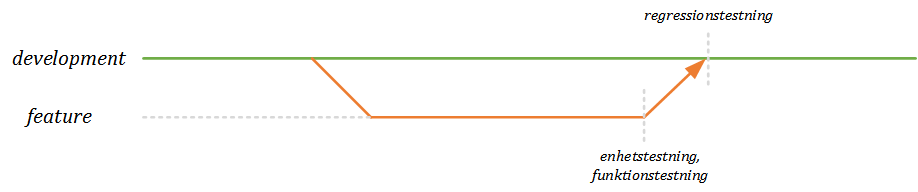
\includegraphics[scale=1]{git_workflow}
  \caption{Illustration över ett tänkt arbetsflöde}
  \label{fig:git_workflow}
\end{figure}
\subsection{Enhetstest}
Enhetstester utförs med hjälp av enhetstestramverket Mocha, tillsammans med biblioteket Chai som ger tillgång till funktionalitet för att validera huruvida funktioners in-/utdata motsvarar förväntade värden. Varje utvecklare är ansvarig för att belägga den incheckade koden med enhetstester. 

\subsection{Funktionstest}
Till varje utvecklad funktionalitet, buggfix eller kodunderhåll formuleras ett testfall. Detta testfall formuleras enligt överenskommet format för att undvika tvetydigheter som kan uppstå mellan testare och utvecklare. Tesfallet utförs av en utvecklare som valts att testa den givna utvecklingsuppgiften, där enhetstest ingår i standardformuleringen för testfall. 

\subsubsection{Utformning av testfall}


\subsection{Regressionstest}


%%%%%%%%%%%%%%%%%%%%%%%%%%%%%%%%%%%%%%%%%%%%%%%%%%%%%%%%%%%%%%%%%%%%%%
%%% lorem.tex ends here

%%% Local Variables: 
%%% mode: latex
%%% TeX-master: "demothesis"
%%% End: 
